\documentclass[11pt,t]{beamer}
\usetheme{metropolis}
\metroset{progressbar=frametitle,numbering=fraction}
\usefonttheme[onlymath]{serif}
\usepackage{bm}
\usepackage{amsmath,amssymb,amsfonts}
\usepackage{booktabs}
\usepackage{graphicx}
\usepackage{xcolor}
\usepackage{tikz}
\usetikzlibrary{calc,positioning}
\graphicspath{{./figures/}}

\newcommand{\rmd}{\mathrm{d}}
\newcommand{\rmi}{\mathrm{i}}
\newcommand{\Tr}{\operatorname{Tr}}

\title{Coarse-to-fine generation of 2D SU(2) gauge fields}
\date{October 2, 2026}
\author{Yang-yang Tan}

\definecolor{burgundy}{RGB}{127, 0, 32}
\definecolor{Kleinblue}{RGB}{0, 47, 167}
\newcommand{\kb}[1]{{\bfseries\color{Kleinblue} #1}}
\makeatletter
\newcommand{\refs}[1]{%
  \begin{tikzpicture}[remember picture, overlay]
    \node[anchor=south west, inner sep=0pt, align=flush left,
          text width=\dimexpr\textwidth-1.4cm\relax]
      at ([xshift=\beamer@leftmargin, yshift=0.6cm]current page.south west)
      {\raggedright\tiny\color{black!65} #1\par};
  \end{tikzpicture}}
\makeatother
\newcommand{\rtag}[1]{\textcolor{burgundy}{\textbf{#1}}}

\tikzset{
  stage/.style={
    rectangle, rounded corners=3pt,
    draw=#1!80, fill=#1!12, line width=0.8pt,
    minimum width=1.9cm, minimum height=1.2cm,
    align=center, font=\scriptsize, text=#1!50!black,
    inner sep=3pt
  },
  tlarrow/.style={
    ->, >=stealth, line width=1.2pt, draw=gray!55,
    shorten >=2pt, shorten <=2pt
  }
}

\begin{document}
\begin{frame}[plain,noframenumbering,t]
  \vspace*{1.6cm}
  {\LARGE\bfseries \inserttitle\par}
  \vspace{0.6em}
  {\color{orange}\rule{\textwidth}{0.4pt}\par}
  \vspace{1.4em}
  {\normalsize\bfseries \insertauthor\par}
  \vspace{0.6em}
  {\small IPI, The University of Tokyo\par}
  \vspace{0.3em}
  {\normalsize \insertdate\par}
\end{frame}

% ----------------------------------------------------------------
\begin{frame}{Diffusion model on SU(2) links}
  \begin{columns}[T,onlytextwidth]
    \begin{column}{0.58\textwidth}
      \small
      \kb{Forward SDE}\quad links $U_\mu(x)\in SU(2)$
      \[
        \rmd U=\rmi\,g(t)\,\rmd w^a\,T^a\,U,\qquad T^a=\tfrac{\sigma^a}{2}
      \]
      \vspace{-0.8em}

      $w^a$ Wiener processes. $\Sigma(t)^2=\int_0^t g^2\,\rmd t'$ is the accumulated variance, Haar at $t=1$.

      \vspace{1.2em}
      \kb{Reverse SDE}\quad from Haar at $t=1$
      \[
        \rmd U=\rmi\big[-g^2s^a\,\rmd t+g\,\rmd\bar w^a\big]T^a\,U
      \]
      \vspace{-0.8em}

      $\bar w^a$ reverse-time Wiener. Score $s^a=\nabla^a\log p_t$, $p_t$ density of $U_t$, $p_0\propto e^{-S_W}$ with Wilson action $S_W$. $\nabla^a$ derivative along $U\to e^{\rmi\epsilon T^a}U$.
    \end{column}
    \begin{column}{0.39\textwidth}
      \small
      \kb{Built-in}\\
      gauge covariance\\
      $s_\mu(x)\to\Omega(x)\,s_\mu(x)\,\Omega(x)^\dagger$\\
      $s_\mu=s_\mu^aT^a$, $\Omega(x)\in SU(2)$

      \vspace{1.2em}
      \kb{Architecture}\\
      L-CNN. Loops $W_c(x)$ at $x$ from transported plaquettes, channel $c$

      \vspace{1.2em}
      \kb{Learned}\\
      gauge-invariant weights $c_{\mu c}$
      \[
        s_\mu^a=\frac{1}{\Sigma(t)}\sum_c c_{\mu c}\,W_c^a
      \]
      \vspace{-0.8em}

      $W_c=W_c^0+\rmi\,W_c^a\sigma^a$
    \end{column}
  \end{columns}
  \refs{\rtag{L-CNN:} Favoni et al., PRL 128, 032003 (2022).}
\end{frame}

% ----------------------------------------------------------------
\begin{frame}{Superresolution}
  \centering
  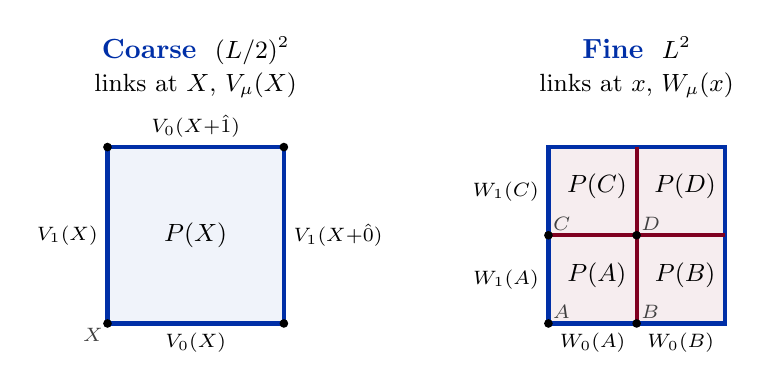
\begin{tikzpicture}[scale=1.12, lab/.style={font=\scriptsize}, site/.style={font=\scriptsize, text=black!75, inner sep=1.5pt}]
    \node[anchor=south, align=center] at (1,2.45) {\kb{Coarse}\ \ {\small $(L/2)^2$}\\ {\small links at $X$, $V_\mu(X)$}};
    \node[anchor=south, align=center] at (6,2.45) {\kb{Fine}\ \ {\small $L^2$}\\ {\small links at $x$, $W_\mu(x)$}};
    \fill[Kleinblue!6] (0,0) rectangle (2,2);
    \draw[line width=1.5pt, Kleinblue] (0,0) rectangle (2,2);
    \foreach \x/\y in {0/0,2/0,0/2,2/2}
      \fill (\x,\y) circle (1.4pt);
    \node[site, anchor=north east] at (0,0) {$X$};
    \node[lab, below] at (1,0) {$V_0(X)$};
    \node[lab, left] at (0,1) {$V_1(X)$};
    \node[lab, right] at (2,1) {$V_1(X{+}\hat0)$};
    \node[lab, above] at (1,2) {$V_0(X{+}\hat1)$};
    \node[font=\small] at (1,1) {$P(X)$};
    \begin{scope}[shift={(5,0)}]
      \fill[burgundy!7] (0,0) rectangle (2,2);
      \draw[line width=1.5pt, Kleinblue] (0,0) rectangle (2,2);
      \draw[line width=1.5pt, burgundy] (0,1) -- (2,1);
      \draw[line width=1.5pt, burgundy] (1,0) -- (1,2);
      \foreach \x/\y in {0/0,1/0,0/1,1/1}
        \fill (\x,\y) circle (1.4pt);
      \node[site, anchor=south west] at (0,0) {$A$};
      \node[site, anchor=south west] at (1,0) {$B$};
      \node[site, anchor=south west] at (0,1) {$C$};
      \node[site, anchor=south west] at (1,1) {$D$};
      \node[lab, below] at (0.5,0) {$W_0(A)$};
      \node[lab, below] at (1.5,0) {$W_0(B)$};
      \node[lab, left] at (0,0.5) {$W_1(A)$};
      \node[lab, left] at (0,1.5) {$W_1(C)$};
      \node[font=\small] at (0.55,0.55) {$P(A)$};
      \node[font=\small] at (1.55,0.55) {$P(B)$};
      \node[font=\small] at (0.55,1.55) {$P(C)$};
      \node[font=\small] at (1.55,1.55) {$P(D)$};
    \end{scope}
  \end{tikzpicture}

  \raggedright
  \vspace{0.5em}
  \small
  Block of $X$\quad $A=2X$,\ $B=A+\hat0$,\ $C=A+\hat1$,\ $D=A+\hat0+\hat1$\\[0.2em]
  $P(X)=V_0(X)\,V_1(X{+}\hat0)\,V_0(X{+}\hat1)^\dagger\,V_1(X)^\dagger$, fine $P(x)$ alike from $W$

  \vspace{0.6em}
  \kb{Constraints}\\[0.2em]
  (i)\ coarse links kept\quad $W_\mu(2X)\,W_\mu(2X+\hat\mu)=V_\mu(X)$\\[0.2em]
  (ii)\ by hand (can be modified)\quad $P(A)=P(B)=P(C)=P(D)\equiv Q$
\end{frame}

% ----------------------------------------------------------------
\begin{frame}{Superresolution, solving the constraints}
  \begin{columns}[T,onlytextwidth]
    \begin{column}{0.56\textwidth}
      \small
      \kb{Choose a gauge}\quad at $B$, $C$, $D$\\
      {\footnotesize\color{black!65} no physical effect}\\[0.3em]
      {\renewcommand{\arraystretch}{1.25}%
      \begin{tabular}{@{}l@{\quad}l@{\quad}l@{}}
        gauge & \multicolumn{2}{@{}l@{}}{$W_0(A)=W_1(A)=W_1(B)=I$}\\
        (i) & \multicolumn{2}{@{}l@{}}{$W_0(B)=V_0$,\ \ $W_1(C)=V_1$}\\
        (ii) & $P(A)=Q$ & $W_0(C)=Q^\dagger$\\
        & $P(B)=Q$ & $W_0(D)=Q^\dagger V_0$\\
        & $P(C)=Q$ & $W_1(D)=Q^2V_1$\\
        & $P(D)=Q$ & $Q^\dagger P(X)\,Q^{-2}=Q$\\
        & \multicolumn{2}{@{}l@{}}{$\Rightarrow\ \alert{Q=P(X)^{1/4}}$, principal root}\\
      \end{tabular}}

      \vspace{0.6em}
      8 links per block $=$ 3 gauge $+$ 2 from (i) $+$ 3 from (ii) at $A$, $B$, $C$.
      (ii) at $D$ then fixes $Q$.

      \vspace{0.4em}
      Covariant under coarse gauge transformations.
    \end{column}
    \begin{column}{0.42\textwidth}
      \centering
      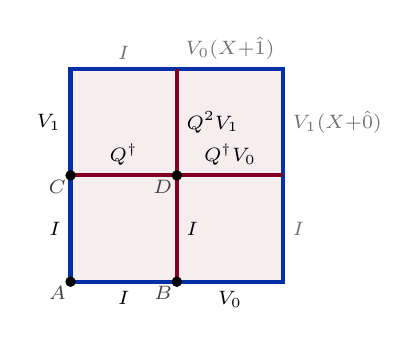
\begin{tikzpicture}[scale=1.35, lab/.style={font=\scriptsize}, nb/.style={font=\scriptsize, text=black!55}, site/.style={font=\scriptsize, text=black!75, inner sep=1.5pt}]
        \fill[burgundy!7] (0,0) rectangle (2,2);
        \draw[line width=1.5pt, Kleinblue] (0,0) -- (2,0) -- (2,2) -- (0,2) -- cycle;
        \draw[line width=1.5pt, burgundy] (0,1) -- (2,1);
        \draw[line width=1.5pt, burgundy] (1,0) -- (1,2);
        \foreach \x/\y in {0/0,1/0,0/1,1/1}
          \fill (\x,\y) circle (1.4pt);
        \node[site, anchor=north east] at (0,0) {$A$};
        \node[site, anchor=north east] at (1,0) {$B$};
        \node[site, anchor=north east] at (0,1) {$C$};
        \node[site, anchor=north east] at (1,1) {$D$};
        \node[lab, below] at (0.5,0) {$I$};
        \node[lab, below] at (1.5,0) {$V_0$};
        \node[lab, left] at (0,0.5) {$I$};
        \node[lab, left] at (0,1.5) {$V_1$};
        \node[lab, above] at (0.5,1) {$Q^\dagger$};
        \node[lab, above] at (1.5,1) {$Q^\dagger V_0$};
        \node[lab, right] at (1,0.5) {$I$};
        \node[lab, right] at (1,1.5) {$Q^2V_1$};
        \node[nb, right] at (2,0.5) {$I$};
        \node[nb, right] at (2,1.5) {$V_1(X{+}\hat0)$};
        \node[nb, above] at (0.5,2) {$I$};
        \node[nb, above] at (1.5,2) {$V_0(X{+}\hat1)$};
      \end{tikzpicture}\\[0.4em]
      {\scriptsize labels are the values of $W_\mu(x)$\\
      $V_\mu\equiv V_\mu(X)$\par}
    \end{column}
  \end{columns}
\end{frame}

% ----------------------------------------------------------------
\begin{frame}{Coarse start}
  \centering
  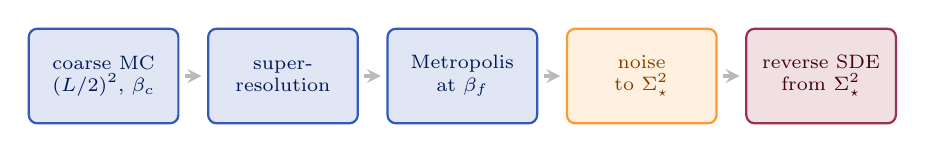
\begin{tikzpicture}[node distance=0.35cm]
    \node[stage=Kleinblue] (c) {coarse MC\\ $(L/2)^2$, $\beta_c$};
    \node[stage=Kleinblue, right=of c] (s) {super-\\resolution};
    \node[stage=Kleinblue, right=of s] (m) {Metropolis\\ at $\beta_f$};
    \node[stage=orange, right=of m] (n) {noise\\ to $\Sigma_\star^2$};
    \node[stage=burgundy, right=of n] (r) {reverse SDE\\ from $\Sigma_\star^2$};
    \draw[tlarrow] (c) -- (s);
    \draw[tlarrow] (s) -- (m);
    \draw[tlarrow] (m) -- (n);
    \draw[tlarrow] (n) -- (r);
  \end{tikzpicture}

  \vspace{0.8em}
  \raggedright
  \begin{columns}[T,onlytextwidth]
    \begin{column}{0.50\textwidth}
      \small
      \kb{Short-distance fluctuations}\\
      Metropolis at $\beta_f$\\[0.3em]
      1.\ 2 sweeps, {\color{burgundy}inner cross} only\\
      2.\ 1 sweep, all links\\
      3.\ random gauge transformation

      \vspace{0.8em}
      \alert{Coarse start below $=$ superresolved field after steps 1, 2, 3}
    \end{column}
    \begin{column}{0.48\textwidth}
      \small
      \kb{Same physical box}\quad $\tfrac{L}{2}a_c=La_f$
      \[
        F(\beta_c)=4F(\beta_f)
      \]
      \vspace{-1.2em}
      \[
        F=a^2\sigma=-\ln\frac{I_2(\beta)}{I_1(\beta)}
      \]
      {\footnotesize
      \begin{tabular}{@{}ll@{}}
        \toprule
        fine & coarse\\
        \midrule
        $32^2$, $\beta_f=2$ & $16^2$, $\beta_c=0.141$\\
        $128^2$, $\beta_f=200$ & $64^2$, $\beta_c=50.37$\\
        \bottomrule
      \end{tabular}}
    \end{column}
  \end{columns}
  \refs{\rtag{String tension:} Detmold et al., arXiv:2101.12668.}
\end{frame}

% ----------------------------------------------------------------
\begin{frame}{Wilson loops at $L=32$}
  \begin{columns}[T,onlytextwidth]
    \begin{column}{0.74\textwidth}
      \includegraphics[width=\linewidth]{su2_L32_reverse_wilson_loops}
    \end{column}
    \begin{column}{0.24\textwidth}
      \small
      Haar, fine and coarse starts at $\Sigma^2=3$ agree.

      \vspace{0.6em}
      All below heat bath, $6\%$ for $W_{2\times2}$.

      \vspace{0.6em}
      Coarse start at $\Sigma^2=1.5$ remembers its start.
    \end{column}
  \end{columns}
\end{frame}

% ----------------------------------------------------------------
\begin{frame}{Action density and string tension at $L=32$}
  \begin{columns}[T,onlytextwidth]
    \begin{column}{0.49\textwidth}
      \includegraphics[width=\linewidth]{su2_L32_reverse_action_density}
    \end{column}
    \begin{column}{0.49\textwidth}
      \includegraphics[width=\linewidth]{su2_L32_reverse_string_tension}
    \end{column}
  \end{columns}

  \vspace{0.8em}
  \small
  $a^2\sigma_{\rm eff}$ from $2\times2$\quad heat bath $0.8356(5)$,\quad Haar $0.8499(6)$

  \vspace{0.4em}
  \alert{Same bias from every start. It is a network error.}
\end{frame}

% ----------------------------------------------------------------
\begin{frame}{Wilson loop fluctuations at $L=32$}
  \begin{columns}[T,onlytextwidth]
    \begin{column}{0.60\textwidth}
      \includegraphics[width=\linewidth]{su2_L32_reverse_second_moments}
    \end{column}
    \begin{column}{0.38\textwidth}
      \small
      \kb{Operator}\\
      $W_{R\times T}(x)=\tfrac12\Tr\,U_{R\times T}(x)$\\
      {\footnotesize $U_{R\times T}(x)$ ordered links around the $R\times T$ loop at $x$}\\[0.3em]
      $\langle W^2\rangle$ average of $W(x)^2$ over $x$ and configurations

      \vspace{0.5em}
      \kb{Exact}\quad infinite volume
      \[
        \langle W^2_{R\times T}\rangle=\tfrac14\big[1+3\,r_1^{RT}\big]
      \]
      \vspace{-1.2em}

      {\footnotesize $r_1=I_3(\beta)/I_1(\beta)$, adjoint channel}

      \vspace{0.5em}
      $1\times1$, $1\times2$ low from all $\Sigma^2=3$ starts.\\
      $2\times2$, $2\times3$ agree within errors.
    \end{column}
  \end{columns}
\end{frame}

% ----------------------------------------------------------------
\begin{frame}{Large Wilson loops at $L=128$}
  \begin{columns}[T,onlytextwidth]
    \begin{column}{0.49\textwidth}
      \includegraphics[width=\linewidth]{su2_L128_reverse_area_law}
    \end{column}
    \begin{column}{0.49\textwidth}
      \includegraphics[width=\linewidth]{su2_L128_reverse_string_tension}
    \end{column}
  \end{columns}

  \vspace{0.8em}
  \small
  \begin{tabular}{@{}l@{\qquad}cccc@{}}
    & exact & Haar & $\Sigma^2=0.2$ & $\Sigma^2=0.02$\\
    $W(1,1)$ & $0.99251$ & $0.99129$ & $0.99215$ & $0.99262$\\
    $W(8,8)$ & $0.618$ & $0.060$ & $0.439$ & $0.616$\\
  \end{tabular}

  \vspace{0.4em}
  \alert{The score alone loses long distances. A coarse start at small $\Sigma^2$ keeps them, with a slightly too ordered plaquette.}
\end{frame}

\end{document}
